In questo capitolo discuteremo della qualità dei dati contenuti nei dataset utilizzati prima e dopo il processo di integrazione; inoltre, proporremo delle analisi descrittive effettuate sui dati integrati. 
\section{Descrizione dei dataset}
I 3 dataset utilizzati, che sono presenti nella \href{https://gitlab.com/Daniele-Papetti/kickstarterprediction}{repository online}, sono stati scaricati dal sito \href{https://www.kaggle.com/}{\emph{www.kaggle.com/}}.
In particolare, due di questi dataset (\textit{countries of the world.csv} e \textit{ks-projects-201612.csv}) sono quelli che verrano utilizzati effettivamente per estrarre delle feature per il processo di apprendimento automatico, mentre il terzo (\textit{country\_code.csv}) viene utilizzato sia come dizionario per l'analisi di qualità dei dati, sia per la parte di integrazione.\\
Il dataset \textit{countries of the world.csv} contiene informazioni che descrivono il rispettivo territorio e sviluppo di 227 nazioni del mondo.
Tra queste si possono trovare informazioni utili come il PIL (GDP) \textit{pro capite}, lo sviluppo in percentuale dei tre settori ed il numero medio di telefoni per abitante; la chiave della relazione è il nome della nazione per esteso.
Invece, \todo[inline]{descrizione kickstarter e poi il perché del terzo dataset DP}
%%% Aggiungerei una descrizione più analitica, tiportamdo sotto forma tabellare nome esatto colonna, tipologia del dato contenuto e descrizione semantica.

\section{Analisi di qualità dei dataset (pre-integrazione)}
\todo[inline]{tutto DP}

\subsection{Accuratezza sintattica attributo country (Figura \ref{fig:dqcountrycodeaccuracy})}

\begin{figure}[h!]
	\centering
	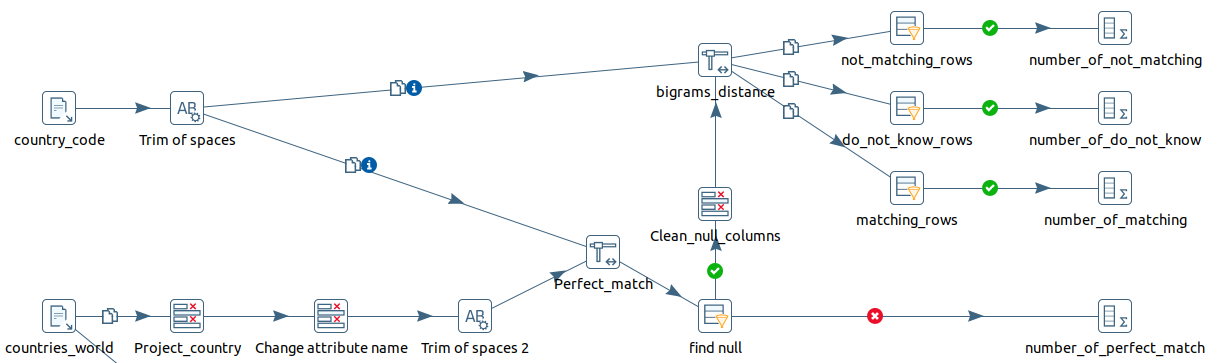
\includegraphics[width=0.7\linewidth]{images/DQ_countrycodeaccuracy}
	\caption{Pipeline per il conteggio delle tuple con codice della country non valido.}
	\label{fig:dqcountrycodeaccuracy}
\end{figure}

\subsection{Accuratezza sintattica attributo state (Figura \ref{fig:dqstateaccuracy})}

\begin{figure}[h!]
	\centering
	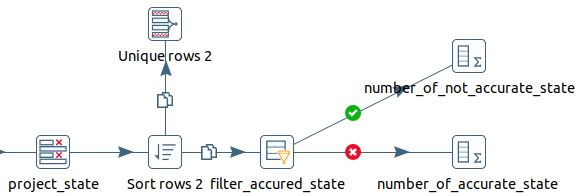
\includegraphics[width=0.7\linewidth]{images/DQ_stateaccuracy}
	\caption{Pipeline che verifica tutti i possibili valori dell'attributo state. Gli unici valori plausibili e accettati dovrebbero essere successful, faild, cancelled, live e suspended.}
	\label{fig:dqstateaccuracy}
\end{figure}


\subsection{Consistenza attributo state (Figura \ref{fig:dqstateaconsistency})}

\begin{figure}[h!]
	\centering
	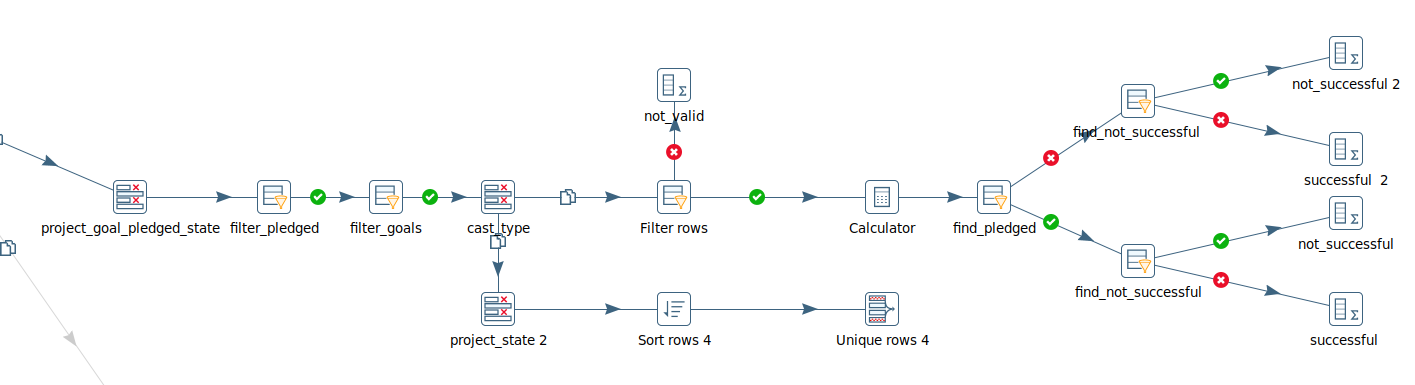
\includegraphics[width=0.7\linewidth]{images/DQ_stateaconsistency}
	\caption{Pipeline per il conteggio delle tuple il cui valore dell'attributo state non è consistente con il totale del denaro raccolto.}
	\label{fig:dqstateaconsistency}
\end{figure}


\subsection{Consistenza attributo backers (Figura \ref{fig:dqbackersconsistency})}

\begin{figure}[h!]
	\centering
	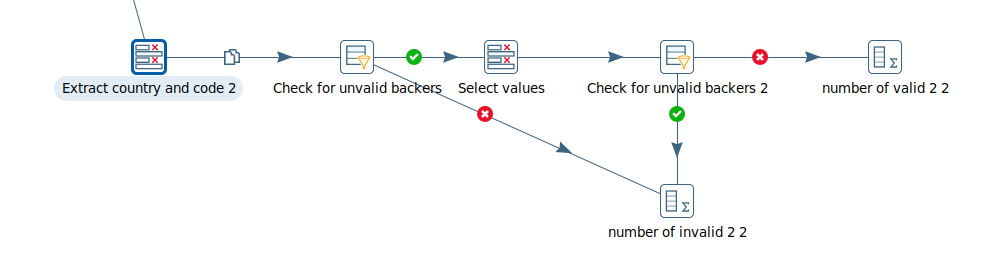
\includegraphics[width=0.7\linewidth]{images/DQ_backersconsistency}
	\caption{Pipeline per il conteggio delle tuple il cui valore dell'attributo backers assume un valore negativo oppure non è consistente con il totale del denaro raccolto.}
	\label{fig:dqbackersconsistency}
\end{figure}


\subsection{Completezza del dataset Kickstarter (Figura \ref{fig:dqcompletezza})}
\todo[inline]{tua parte}
La profilazione dei dati eseguita in precedenza ha mostrato possibili casi di valori sintatticamente corretti ma semanticamente errati; in particolare, un piccolo sottoinsieme di tuple (circa 500) ha mostrato valori privi di senso in diversi campi. Questo sottoinsieme di tuple è stato rimosso dalle operazioni di trasformazione eseguite successivamente, ed è quindi stato deciso di non includere il conteggio di queste tuple nell'analisi della completezza

\begin{figure}[h!]
	\centering
	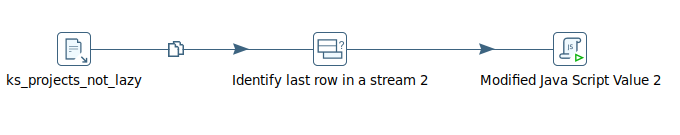
\includegraphics[width=0.7\linewidth]{images/DQ_completezza}
	\caption{Pipeline che utilizza uno script Javascript custom che itera sui campi del dataset e conta il numero di tuple con valore dell'attributo nullo.}
	\label{fig:dqcompletezza}
\end{figure}


\subsection{Accessibilità dei dataset}
Tutti i dataset analizzati mostrano un ottimo livello di accessibilità da parte dell'utente, con nomi degli attributi auto-esplicativi e facile reperibilità dei dati di interesse. Per questo motivo, non si è resa necessaria la creazione di viste sugli schemi locali dei dataset, mantenendo inalterata la struttura di questi ultimi.

\subsection{Porprietà temporali}
Il dataset \textit{ks-projects-201612.csv} contiene tutti i progetti registrati sulla piattaforma Kickstarter fino alla fine del 2016. Il dataset \textit{countries of the world.csv} contiene invece statistiche sugli stati che si riferiscono all'anno 2017. Ne consegue che i dati non siano perfettamente coerenti dal punto di vista temporale, ma abbiamo reputato questo sfasamento marginale, considerata l'assenza di modifiche radicali degli indici statistici presi in considerazioni negli anni consecutivi.

\section{Processo di integrazione dei dati}
Al fine di produrre un dataset integrato per il processo di Machine Learning, si è reso necessario unire i tre dataset scelti in un unico schema integrato. Prima di fare ciò, sfruttando le considerazioni fatte nella parte di analisi di qualità dei dati, sono state eseguite una serie di operazioni di pulizia e raffinamento dei dati.\\

\begin{figure}
	\hspace*{-1cm}%
	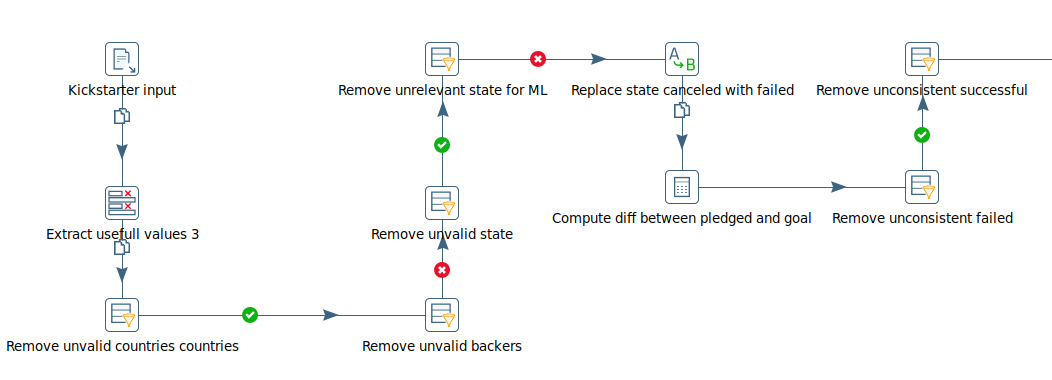
\includegraphics[width=\dimexpr\textwidth+2cm\relax]{images/transformation_kick}%
	\hspace*{-1cm}%
	\caption{Pipeline di trasformazione per il dataset contenente i dati dei progetti Kickstarter}
	\label{fig:transformationkick}
\end{figure}

\subsection{Dataset Kickstarter}
Inizialmente sono stati eliminati tutti quegli attributi che non avevano alcuna informazione rilevante ai fini del training del modello di Machine Learning (Data di creazione e di terminazione, nome, moneta utilizzata \dots).\\
In seguito sono stati rimossi tutti quei record il cui campo relativo alla nazione di origine violasse la rappresentazione standard, ovvero due lettere dell'alfabeto maiuscole. Ciò si è reso necessario in quanto l'analisi della accuratezza sintattica sul campo aveva mostrato una serie di valori privi di significato.\\
Sono stati poi rimossi una serie di record che creavano problemi di consistenza per quanto riguarda il campo dei sostenitori e del totale raccolto. Le analisi condotte in precedenza avevano infatti rilevato che alcuni record avevano un numero di sostenitori negativo, oppure un numero di sostenitori pari a zero, ma il campo che rappresenta l'ammontare del denaro raccolto non era zero anch'esso.\\
E' stata poi condotta una operazione di raffinazione sul campo \textit{state} del dataset, che rappresenta lo stato in cui il progetto si trova. Dopo aver rimosso tutti i valori sintatticamente privi di senso, abbiamo deciso di rimuovere tutti i record il cui stato fosse live, ovvero ancora in corso, oppure suspended, ovvero bloccati dalla piattaforma Kickstarter per violazioni dei termini contrattuali. Questa decisione è stata presa in quanto questo tipo di record potrebbe influenzare negativamente le performance del modello di Machine Learnig, fornendo tuple con uno stato di dubbio significato.
E' stato poi deciso di rendere tutti i record con il campo state uguale a canceled, ovvero cancellati dal creatore, come progetti falliti.\\
Infine, sono stati rimossi tutti i record che mostravano inconsistenza tra lo stato del progetto e la differenza tra denaro richiesto e denaro raccolto. E' infatti mandatorio che se è stato raccolto più denaro di quanto richiesto, il progetto risulti completato, mentre se non sono stati raccolti fondi sufficienti, il progetto risulti fallito.\\
L'intera pipeline di trasformazione è riportata in Figura \ref{fig:transformationkick}.


\subsection{Countries}
Siccome il dataset contenente i dettagli sui progetti Kickstarter sfrutta il codice di 2 lettere per rappresentare la nazione di origine del progetto, mentre il dataset con le informazioni circa il livello di sviluppo dei vari paesi sfrutta il nome completo, è stato necessario individuare un terzo dataset da utilizzare come una tabella di join, in modo da associare ogni nome per esteso con il relativo codice di due lettere.\\
Il dataset individuato per questo scopo si è però rivelato utilizzare una differente sintassi per rappresentare il nome per esteso dei paesi. Per questo motivo, sono state applicate delle tecniche di record linkage per individuare i record corrispondenti ed uniformare la sintassi di questi. Per fare ciò, sono stati utilizzati i dati prodotti dal processo di analisi di qualità dei dati (trattato nella prima parte di questo documento).\\
In particolare, sono stati ignorati i record di perfect match prodotti dalla distanza di edit con soglia zero, mentre sono stati confrontati caso per caso i risultati prodotti dall'analisi tramite bigram. Ponendo la soglia di match a 0.7 e la soglia di non match a 0.5, la soluzione proposta ha prodotto performance ottime, individuando correttamente tutti i match (20/20), e buona parte dei non match(7/11). La presenza di casi limite, quali rappresentazioni radicalmente diverse di un medesimo record, ha reso necessario la supervisione manuale per un piccolo sottoinsieme di questi record.\\

\begin{figure}
	\centering
	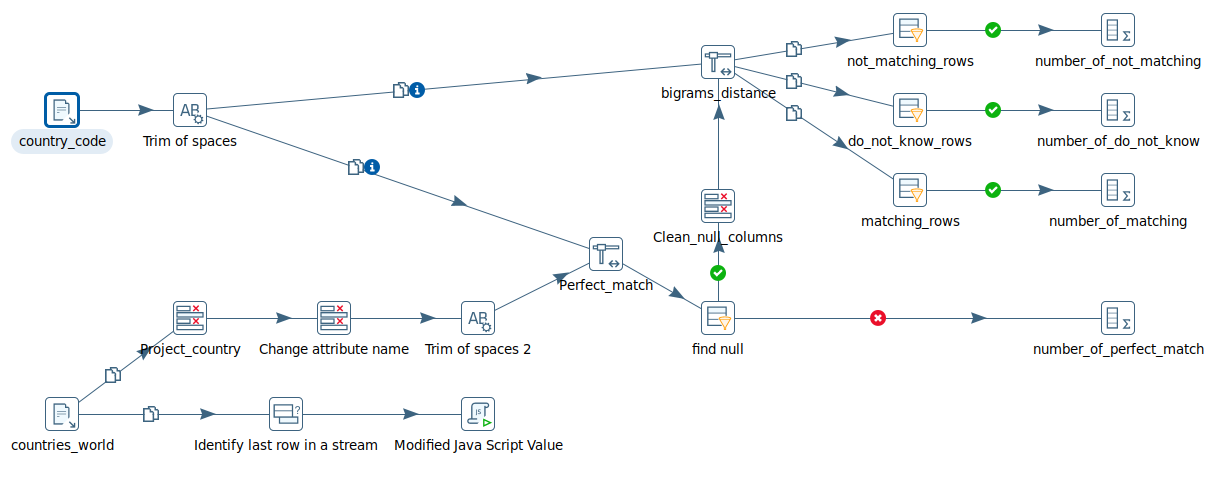
\includegraphics[width=0.7\linewidth]{images/RecordLinkage}
	\caption{Pipeline eseguita per realizzare le operazioni di record linkage}
	\label{fig:recordlinkage}
\end{figure}


\section{Produzione dataset integrato}
A seguito del processo di raffinamento e integrazione dei dataset esposto in precedenza, i tre database sono stati uniti in un unica tabella tramite delle operazioni di merge join, per motivi di efficienza.\\
A seguito dell'unione, sono stati prodotti due nuovi dataset (come mostrato in Figura \ref{fig:transformationcomplete}), uno contenente tutti gli attributi risultanti dalle operazioni precedenti, mentre l'altro epurato da tutti gli attributi privi di valore ai fini dell'addestramento del modello di Machine Learning.

\begin{figure}[p!]
	\centering
	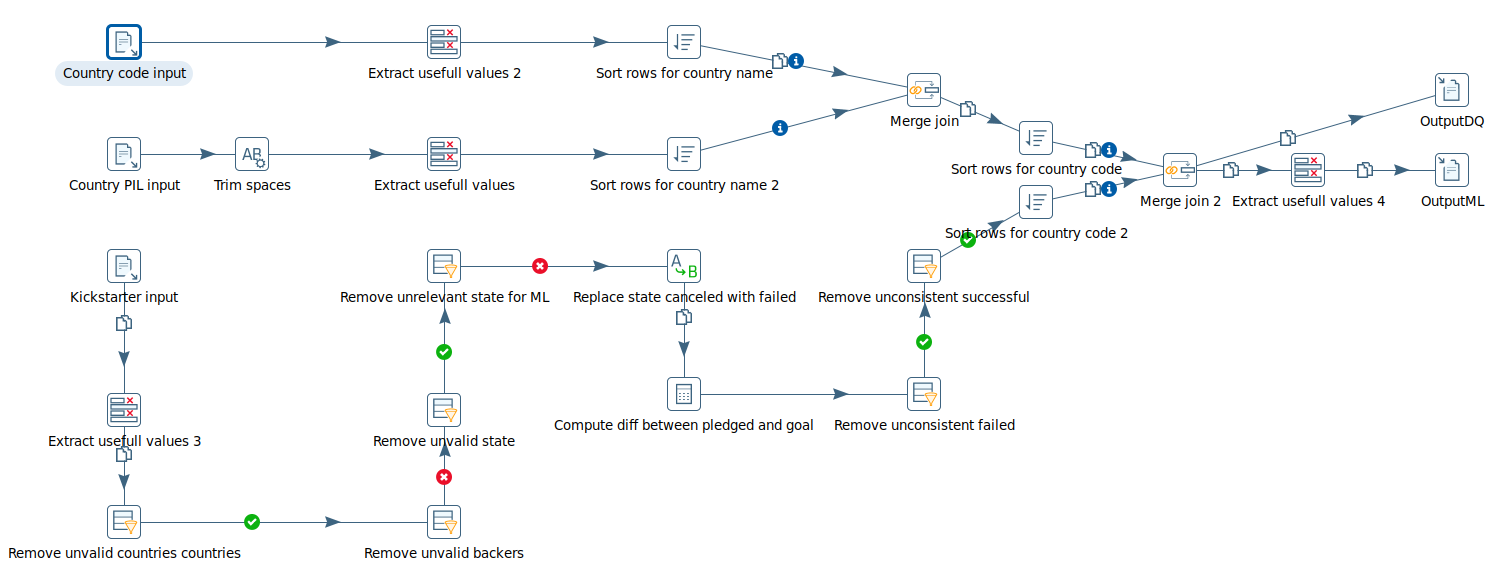
\includegraphics[angle=90,origin=c,width=0.55\linewidth]{images/transformation_complete}
	\caption{Pipeline di trasformazione per il dataset contenente i dati dei progetti Kickstarter}
	\label{fig:transformationcomplete}
\end{figure}

\newpage
\section{Analisi di qualità dei dataset (post-integrazione)}
Al fine di valutare la qualità del lavoro svolto nella fase di integrazione del dataset, le misure di qualità precedentemente stabilite sono state applicate al dataset integrato. In questa sezione verranno riportati i risultati ottenuti e relative considerazioni.

\subsection{Accuratezza sintattica attributo country (Figura \ref{fig:dqtcountries})}
L'attributo presenta 21 possibili valori, tutti formati da una coppia di 2 lettere maiuscole dell'alfabeto. Non sono presenti tuple con valore dell'attributo che violino questo vincolo sintattico.

\begin{figure}[h!]
	\centering
	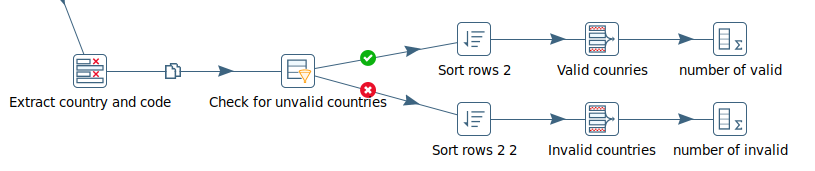
\includegraphics[width=1\linewidth]{images/DQT_countries}
	\caption{Pipeline per la verifica della accuratezza sintattica dell'attributo country}
	\label{fig:dqtcountries}
\end{figure}


\subsection{Accuratezza sintattica attributo state (Figura \ref{fig:dqtstate})}
L'attributo state risulta assumere due possibili valori, successful e failed. Le trasformazioni applicate producono quindi una riduzione dei possibili valori da 408 a 2 possibili valori.

\subsection{Consistenza attributo state (Figura \ref{fig:dqtstate})}
Per l'attributo in esame, non sono presenti tuple inconsistenti, ove il totale raccolto non sia consistente con lo stato del progetto.

\begin{figure}[h!]
	\centering
	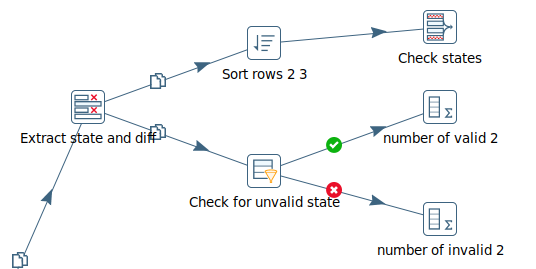
\includegraphics[width=0.6\linewidth]{images/DQT_state}
	\caption{Pipeline per la verifica della consistenza e della accuratezza sintattica dell'attributo state}
	\label{fig:dqtstate}
\end{figure}

\subsection{Consistenza attributo backers (Figura \ref{fig:dqtbackers})}
Per il campo backers, non sono state rilevate tuple con valore del campo negativo oppure con un valore non consistente con totale del denaro raccolto

\begin{figure}[h!]
	\centering
	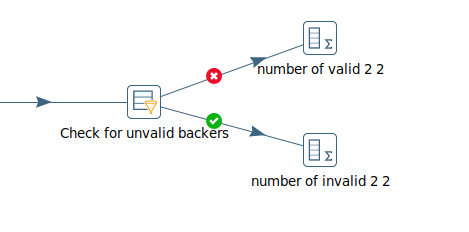
\includegraphics[width=0.7\linewidth]{images/DQT_backers}
	\caption{Pipeline per la verifica della consistenza dell'attributo backers}
	\label{fig:dqtbackers}
\end{figure}

\subsection{Completezza del dataset}
Ai fini di valutare la completezza del dataset prodotto, è stato eseguito nuovamente lo script che ricerca e conta i campi nulli presenti del dataset. L'esecuzione di questo processo conferma l'assenza di campi nulli nel dataset prodotto.

\subsection{Accessibilità del dataset}
Al fine di garantire una accessibilità ottimale al dataset sfruttato per eseguire il training del modello di Machine Learning, sono stati selezionati nomi significativi ed autoesplicativi per le gli attributi rappresentati nel dataset.

\subsection{Porprietà temporali}
Le considerazioni rimangono analoghe a quelle effettuate prima delle operazioni di integrazione dei dati.

\subsection{Altre misure di qualità}
Al fine di verificare l'efficacia dell'operazione di record linkage e data fusion (eseguite a mano) compiute sul campo country del dataset \textit{countries of the world.csv}, sono state nuovamente misurate le distanze con il campo country\_name del dataset \textit{country\_code.csv}. Questa misura, eseguita mediante la pipeline riportata in Figura \ref{fig:qdtrecordlinkage}, mostrano come il nome dei perfect match sia aumentato a seguito delle modifche apportate al dataset \textit{countries of the world.csv}. Allo stesso modo, sfruttando le bigrams, all'interno degli insiemi di incertezza e di non match, sono rimaste solo le coppie che effettivamente non dovevano essere linkate, mentre quelle rilevate come match nella prima analisi sono state tutte portate ad essere perfect match.

\begin{figure}[h!]
	\centering
	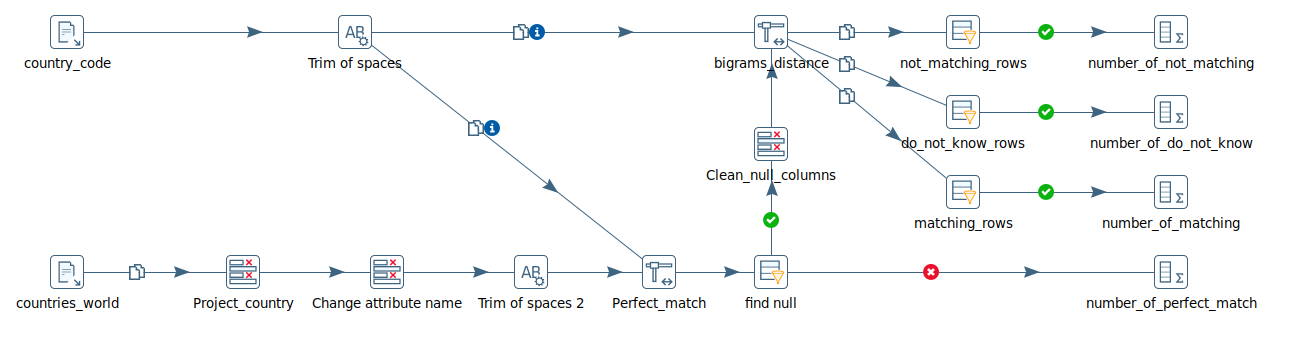
\includegraphics[width=1\linewidth]{images/QDT_recordlinkage}
	\caption{Pipeline utilizzata per la verifica del processo di record linkage effettuata}
	\label{fig:qdtrecordlinkage}
\end{figure}

\captionof{table}{Tabella riassuntiva che mostra il numero di tuple che non soddisfano i vincoli di consistenza o di accuratezza sintattica prima e dopo le trasformazioni applicate}

\begin{tabular}{|c|c|c|}
	\hline 
	Misura & Pre-trasformazione & Post-trasformazione \\ 
	\hline 
	Accuratezza sintattica state & 404 & 0 \\ 
	\hline 
	Consistenza state & 524 & 0 \\ 
	\hline 
	Accuratezza sintattica country code & 141 & 0 \\ 
	\hline 
	Consistenza backers & 3703 & 0 \\ 
	\hline 
	Completezza tabella & 3795 & 0 \\ 
	\hline 
\end{tabular} 

